\documentclass[10pt,a4paper]{article}
\usepackage[a4paper,margin=2.2cm]{geometry}
\usepackage[T1]{fontenc}
\usepackage{lmodern}
\usepackage{microtype}
\usepackage{amsmath,amssymb}
\usepackage{graphicx}
\usepackage{booktabs,tabularx,longtable,array}
\usepackage[table]{xcolor}
\usepackage{caption}
\usepackage{enumitem}
\usepackage{tikz}
\usepackage[section]{placeins}
\usepackage{needspace}
\usepackage{float}
\usetikzlibrary{arrows.meta,positioning}
\usepackage[colorlinks=true,linkcolor=blue!50!black,urlcolor=blue!50!black,citecolor=blue!50!black]{hyperref}
\graphicspath{{../figures/}}
\setlist{nosep,leftmargin=1.4em}
\captionsetup{font=small,labelfont=bf}
\renewcommand{\arraystretch}{1.15}
\newcommand{\FsI}{4.00}
\newcommand{\NfftI}{256}
\newcommand{\NcpI}{64}
\newcommand{\NusedI}{200}
\newcommand{\DfI}{15.625}
\newcommand{\TsymI}{80.0}
\newcommand{\SymRateI}{12.500}
\newcommand{\BoccI}{3.14}
\newcommand{\RresI}{95.5}
\newcommand{\RcpI}{4.20}
\newcommand{\RambI}{19.2}
\newcommand{\NsymI}{13106}
\newcommand{\TcpiI}{1048.5}
\newcommand{\DresI}{0.95}
\newcommand{\DmaxI}{6.25}
\newcommand{\VresI}{0.117}
\newcommand{\GprocI}{64.2}
\newcommand{\NoiseI}{\textminus 102.0}
\newcommand{\UsbI}{16}
\newcommand{\BufI}{163840}
\newcommand{\BufMsI}{41.0}
\newcommand{\BufRateI}{24.4}
\newcommand{\PaprI}{11.1}
\newcommand{\PtxI}{\textminus 15.0}
\newcommand{\GantI}{6}
\newcommand{\NFI}{6}
\newcommand{\IsoI}{20}
\newcommand{\LvlI}{\textminus 15}
\newcommand{\FsO}{30.72}
\newcommand{\NfftO}{1024}
\newcommand{\NcpO}{128}
\newcommand{\NusedO}{800}
\newcommand{\DfO}{30.000}
\newcommand{\TsymO}{37.5}
\newcommand{\SymRateO}{26.667}
\newcommand{\BoccO}{24.03}
\newcommand{\RresO}{12.5}
\newcommand{\RcpO}{1.17}
\newcommand{\RambO}{10.0}
\newcommand{\NsymO}{3639}
\newcommand{\TcpiO}{136.5}
\newcommand{\DresO}{7.33}
\newcommand{\DmaxO}{13.33}
\newcommand{\VresO}{0.897}
\newcommand{\GprocO}{64.6}
\newcommand{\NoiseO}{\textminus 93.1}
\newcommand{\UsbO}{123}
\newcommand{\BufO}{589824}
\newcommand{\BufMsO}{19.2}
\newcommand{\BufRateO}{52.1}
\newcommand{\PaprO}{10.9}
\newcommand{\PtxO}{\textminus 5.0}
\newcommand{\GantO}{12}
\newcommand{\NFO}{6}
\newcommand{\IsoO}{25}
\newcommand{\LvlO}{\textminus 15}
\newcommand{\LambdaCm}{12.24}
\newcommand{\RmsI}{\textminus 12.1}
\newcommand{\RmsO}{\textminus 11.7}
\newcommand{\Fc}{2.45}
\newcommand{\PdpI}{\textminus 75.3}
\newcommand{\LbPWalk}{\textminus 89.6}
\newcommand{\LbSWalk}{12.3}
\newcommand{\LbGWalk}{76.5}
\newcommand{\LbDWalk}{14.4}
\newcommand{\LbPFan}{\textminus 91.7}
\newcommand{\LbSFan}{10.3}
\newcommand{\LbGFan}{74.5}
\newcommand{\LbDFan}{16.4}
\newcommand{\LbPRoom}{\textminus 66.2}
\newcommand{\LbSRoom}{35.7}
\newcommand{\LbGRoom}{99.9}
\newcommand{\LbDRoom}{\textminus 9.1}
\newcommand{\PdpO}{\textminus 66.2}
\newcommand{\LbPUav}{\textminus 126.8}
\newcommand{\LbSUav}{\textminus 33.7}
\newcommand{\LbGUav}{30.9}
\newcommand{\LbDUav}{60.6}
\newcommand{\LbPPers}{\textminus 102.7}
\newcommand{\LbSPers}{\textminus 9.6}
\newcommand{\LbGPers}{55.1}
\newcommand{\LbDPers}{36.5}
\newcommand{\LbPClut}{\textminus 95.1}
\newcommand{\LbSClut}{\textminus 2.0}
\newcommand{\LbGClut}{62.6}
\newcommand{\LbDClut}{28.9}
\newcommand{\WalkDT}{18.35}
\newcommand{\WalkDE}{18.33}
\newcommand{\WalkDErr}{\textminus 0.018}
\newcommand{\WalkDErrC}{\textminus 0.019}
\newcommand{\WalkRT}{8.55}
\newcommand{\WalkRE}{8.44}
\newcommand{\WalkSnr}{54.8}
\newcommand{\FanT}{60.0}
\newcommand{\FanE}{60.00}
\newcommand{\BerI}{0}
\newcommand{\BitsI}{5{,}115{,}600}
\newcommand{\EvmI}{\textminus 25.0}
\newcommand{\AdcI}{\textminus 3.3}
\newcommand{\NdetI}{26}
\newcommand{\UavRT}{178.89}
\newcommand{\UavRE}{178.68}
\newcommand{\UavRErr}{\textminus 0.21}
\newcommand{\UavRErrC}{\textminus 0.017}
\newcommand{\UavDT}{103.34}
\newcommand{\UavDE}{102.95}
\newcommand{\UavDErr}{\textminus 0.40}
\newcommand{\UavDErrC}{\textminus 0.054}
\newcommand{\UavSnr}{27.3}
\newcommand{\UavVT}{\textminus 12.65}
\newcommand{\UavVE}{\textminus 12.60}
\newcommand{\UavBrMin}{193.3}
\newcommand{\UavBrMax}{208.3}
\newcommand{\UavBrE}{201.0}
\newcommand{\PersDT}{3.67}
\newcommand{\PersDE}{6.97}
\newcommand{\PersDErr}{+3.29}
\newcommand{\PersRT}{93.37}
\newcommand{\PersRE}{93.37}
\newcommand{\BerO}{0}
\newcommand{\BitsO}{5{,}644{,}800}
\newcommand{\EvmO}{\textminus 24.9}
\newcommand{\GenieSame}{identical}
\newcommand{\NdetO}{7}
\newcommand{\TwoCfoT}{4900.0}
\newcommand{\TwoCfoE}{4900.007}
\newcommand{\TwoCfoErr}{+0.007}
\newcommand{\TwoLw}{0.01}
\newcommand{\TwoDT}{18.33}
\newcommand{\TwoRT}{8.48}
\newcommand{\TwoBerNone}{0.50}
\newcommand{\TwoWalkNone}{missed}
\newcommand{\TwoCfoOnlyR}{81.4}
\newcommand{\TwoCfoOnlyRErr}{+73.0}
\newcommand{\TwoCfoOnlySnr}{19.2}
\newcommand{\TwoRefD}{18.31}
\newcommand{\TwoRefDErr}{\textminus 0.023}
\newcommand{\TwoRefR}{8.14}
\newcommand{\TwoRefRErr}{\textminus 0.34}
\newcommand{\TwoRefSnr}{28.0}
\newcommand{\TwoRefBer}{0}
\newcommand{\TwoOneBer}{0}
\newcommand{\TwoCfoOnlyBer}{0}
\newcommand{\TwoOneSnr}{57.2}
\newcommand{\TwoOneD}{18.32}
\newcommand{\TwoOneDErr}{\textminus 0.014}
\newcommand{\SensHead}{0.001 & 0.01 & 0.1 & 0.3 & 1 & 3}
\newcommand{\SensRows}{100 ms & 38.3 & 30.6 & 20.4 & 16.7 & missed & missed \\
20 ms & 29.8 & 27.6 & 21.0 & 19.2 & 16.6 & 14.2 \\}
\newcommand{\McRows}{50 & 1.00 & 41.2 & 40.8 & 0.06 & 1.71 \\
100 & 1.00 & 30.0 & 26.1 & 0.35 & 0.68 \\
150 & 1.00 & 22.9 & 18.5 & 0.81 & 0.51 \\
200 & 1.00 & 17.9 & 13.7 & 1.50 & 0.92 \\
250 & 0.25 & 14.1 & 12.2 & 2.06 & 1.84 \\
300 & 0.08 & 10.9 & 12.1 & 1.05 & 0.28 \\
400 & 0.00 & 5.9 & -- & -- & -- \\}
\newcommand{\McTrials}{12}

\newcommand{\code}[1]{\texttt{#1}}
\newcolumntype{L}{>{\raggedright\arraybackslash}X}

\title{\textbf{Bistatic OFDM Integrated Sensing and Communication\\with a PlutoSDR and GNU Radio}\\[4pt]
\large Design, simulation and software validation}
\author{Amirreza Piri}
\date{Technical report, version 1.0, 5 November 2026}

\begin{document}
\maketitle


\begin{abstract}
\noindent One OFDM waveform is used for two tasks at once: it carries QPSK data, which the receiver decodes
without prior knowledge of the payload, and it illuminates the scene for a bistatic radar that estimates
range-sum and Doppler. The receiver uses the reciprocal-filter OFDM radar method with a decision-directed
reference, direct-path delay calibration, zero-Doppler clutter suppression, ordered-statistic CFAR and a rotor
line-spacing estimator for micro-Doppler. For two independent SDRs it adds blind cyclic-prefix CFO estimation
and direct-path referencing. Two operating points are designed around the PlutoSDR's limits: an indoor mode
(\FsI\,MS/s, \BoccI\,MHz, \TcpiI\,ms CPI, \DresI\,Hz Doppler resolution) and an outdoor UAV mode (\FsO\,MS/s,
\BoccO\,MHz, \RresO\,m range-sum resolution). In simulation the indoor walker's torso Doppler is estimated with
an error of \WalkDErr\,Hz, a fan's rotor-line spacing as \FanE\,Hz (truth \FanT\,Hz), and a quadcopter's excess
range-sum and Doppler with errors of \UavRErr\,m and \UavDErr\,Hz, all with zero bit errors on the same waveform.
\end{abstract}

\setcounter{tocdepth}{1}
\tableofcontents

%======================================================================================
\section{Scope and contributions}
\begin{itemize}
\item A complete OFDM integrated sensing and communication (ISAC) chain for the ADALM-PLUTO (AD9363):
waveform, synchronisation, communication receiver, OFDM radar, CFAR, micro-Doppler.
\item A bistatic channel simulator with a physical link budget and SDR impairments (timing offset, CFO, SFO, LO
phase noise, thermal noise, 12-bit ADC with clipping), used to verify every estimator against ground truth.
\item GNU Radio~3.10 flowgraphs (live one-Pluto ISAC, TX node, RX recorder, headless replay) built around one
embedded Python block; a \code{pyadi-iio} capture script recording contiguous CPIs as SigMF; import of SDR++
baseband WAV recordings.
\item A test suite of %%N_TESTS%%tests, including runs of the flowgraph in the GNU Radio runtime.
\end{itemize}

%======================================================================================
\section{System overview}
\begin{figure}[htbp]
\centering
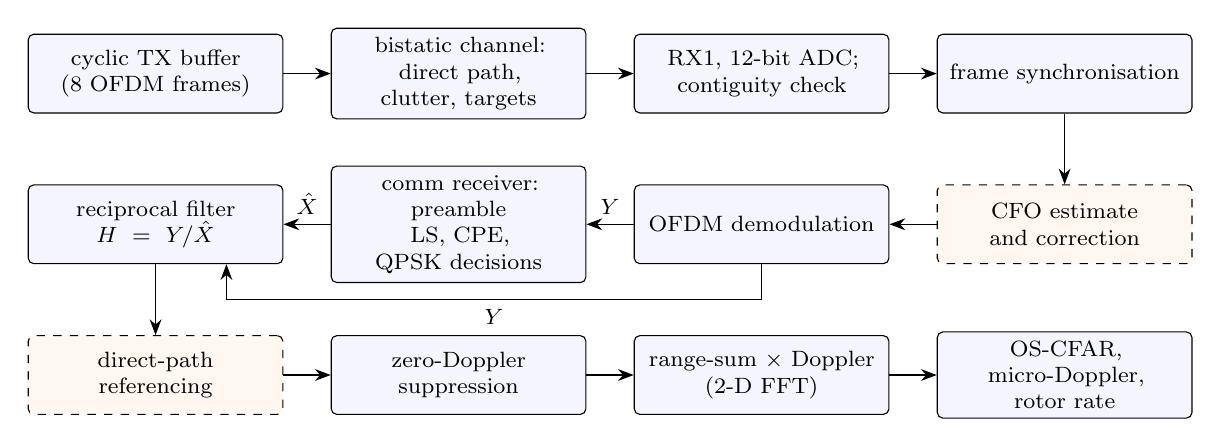
\begin{tikzpicture}[node distance=9mm and 6mm, every node/.style={font=\footnotesize},
  box/.style={draw, rounded corners=2pt, align=center, minimum height=10mm, text width=30mm, fill=blue!4},
  opt/.style={box, dashed, fill=orange!6},
  arr/.style={-{Stealth[length=2mm]}}]
% row 1: left to right
\node[box] (tx) {cyclic TX buffer\\(8 OFDM frames)};
\node[box, right=of tx] (ch) {bistatic channel:\\direct path, clutter, targets};
\node[box, right=of ch] (rx) {RX1, 12-bit ADC;\\contiguity check};
\node[box, right=of rx] (sync) {frame synchronisation};
% row 2: right to left
\node[opt, below=of sync] (cfo) {CFO estimate\\and correction};
\node[box, left=of cfo] (dem) {OFDM demodulation};
\node[box, left=of dem] (comm) {comm receiver: preamble\\LS, CPE, QPSK decisions};
\node[box, left=of comm] (rf) {reciprocal filter\\$H = Y/\hat X$};
% row 3: left to right
\node[opt, below=of rf] (ref) {direct-path\\referencing};
\node[box, right=of ref] (zd) {zero-Doppler\\suppression};
\node[box, right=of zd] (rd) {range-sum $\times$ Doppler\\(2-D FFT)};
\node[box, right=of rd] (cfar) {OS-CFAR, micro-Doppler,\\rotor rate};
\draw[arr] (tx)--(ch); \draw[arr] (ch)--(rx); \draw[arr] (rx)--(sync); \draw[arr] (sync)--(cfo);
\draw[arr] (cfo)--(dem); \draw[arr] (dem)--node[above]{$Y$}(comm); \draw[arr] (comm)--node[above]{$\hat X$}(rf);
\draw[arr] (dem.south) -- ++(0,-4.5mm) -| node[pos=0.25,below]{$Y$} ([xshift=9mm]rf.south);
\draw[arr] (rf)--(ref); \draw[arr] (ref)--(zd); \draw[arr] (zd)--(rd); \draw[arr] (rd)--(cfar);
\end{tikzpicture}
\caption{Processing chain. Dashed boxes are only used with two separate SDRs (independent clocks).}
\label{fig:chain}
\end{figure}

\noindent \textbf{One-Pluto mode.} TX1 and RX1 of one PlutoSDR drive two antennas 3--10\,m apart over cables. The
geometry is bistatic; the clock is shared (no CFO or SFO), which is the role that fibre synchronisation plays
in a distributed MIMO testbed. \textbf{Two-Pluto mode.} The TX and RX nodes have independent TCXOs; the receiver
estimates and removes the synchronisation errors (Section~\ref{sec:sync}). Fig.~\ref{fig:geom} shows the two
simulated scenes.

\begin{figure}[htbp]
\centering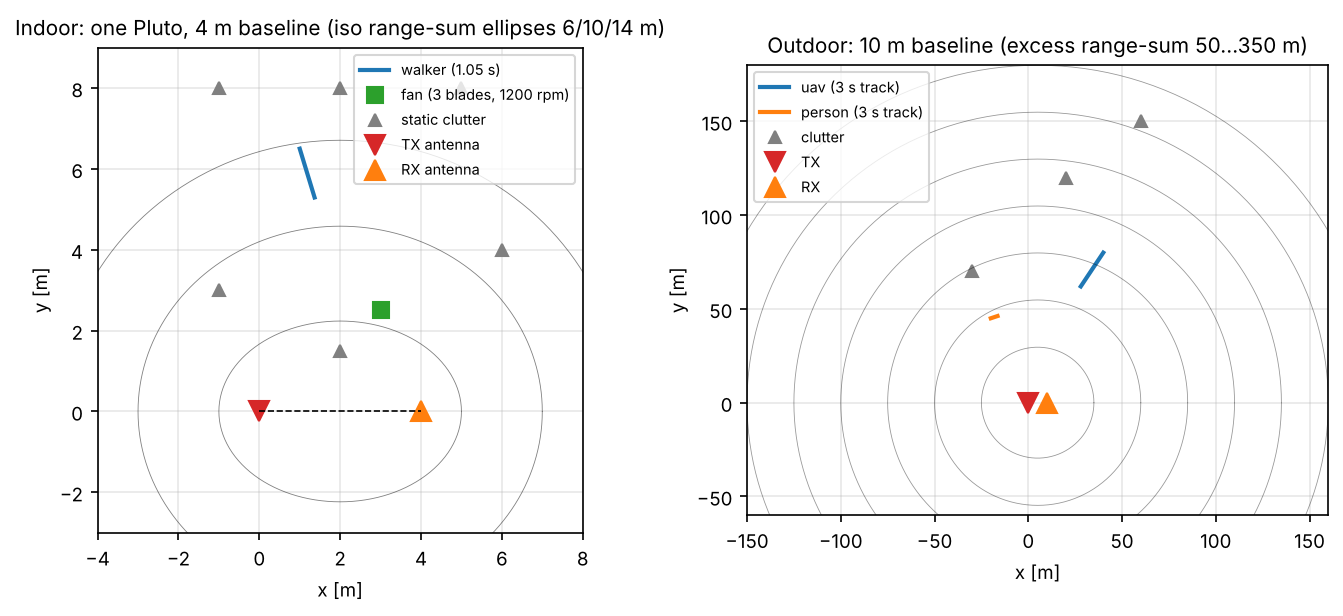
\includegraphics[width=\linewidth]{fig01_geometry.png}
\caption{Simulated geometries. Left: indoor, 4\,m baseline. Right: outdoor, 10\,m baseline, iso-range-sum
ellipses every 50\,m of excess range-sum.}
\label{fig:geom}
\end{figure}

%======================================================================================
\section{Waveform and numerology}
CP-OFDM with QPSK data. Every frame of 64 symbols starts with a Zadoff--Chu preamble (prime length $\ge N_{used}$,
truncated to $N_{used}$, constant modulus). Frame~0 uses root 25 and frames 1--7 use root 34, so the receiver can
locate the start of the cyclic buffer. The DC subcarrier is empty. The cyclic TX buffer holds 8 frames with
different payloads (Section~\ref{sec:impl}).

\begin{table}[htbp]
\centering\small
\caption{Numerology (from \code{config/*.yaml} via \code{isac/config.py}). $\lambda=\LambdaCm$\,cm at $f_c=\Fc$\,GHz.}
\label{tab:num}
\begin{tabular}{lccl}
\toprule
Quantity & Indoor & Outdoor UAV & Definition\\
\midrule
Sample rate $f_s$ & \FsI\,MS/s & \FsO\,MS/s & \\
FFT size / CP & \NfftI\ / \NcpI & \NfftO\ / \NcpO & samples\\
Used subcarriers & \NusedI & \NusedO & DC empty\\
Subcarrier spacing $\Delta f$ & \DfI\,kHz & \DfO\,kHz & $f_s/N$\\
Symbol period $T$ (incl.\ CP) & \TsymI\,\textmu s & \TsymO\,\textmu s & slow-time rate \SymRateI\ / \SymRateO\,kHz\\
Occupied bandwidth $B$ & \BoccI\,MHz & \BoccO\,MHz & $(N_{used}+1)\Delta f$\\
Range-sum resolution & \RresI\,m & \RresO\,m & $c/B$\\
ISI-free excess range-sum & \RcpI\,km & \RcpO\,km & $c\,(N_{cp}-b)/f_s$, back-off $b=8$\\
Unambiguous excess range-sum & \RambI\,km & \RambO\,km & $c/\Delta f$\\
Symbols per CPI / CPI & \NsymI\ / \TcpiI\,ms & \NsymO\ / \TcpiO\,ms & $2^{22}$ samples\\
Doppler resolution & \DresI\,Hz & \DresO\,Hz & $1/T_{CPI}$\\
Range-sum-rate resolution & \VresI\,m/s & \VresO\,m/s & $\lambda/T_{CPI}$\\
Unambiguous Doppler & $\pm$\DmaxI\,kHz & $\pm$\DmaxO\,kHz & $\pm 1/(2T)$\\
2-D coherent processing gain & \GprocI\,dB & \GprocO\,dB & $10\log_{10}(N_{used}N_{sym})$\\
USB~2.0 load if streamed & \UsbI\,MB/s & \UsbO\,MB/s & $4f_s$ (int16 I/Q)\\
Cyclic TX buffer & \BufI\ (\BufMsI\,ms) & \BufO\ (\BufMsO\,ms) & repeats at \BufRateI\ / \BufRateO\,Hz\\
PAPR of the TX buffer & \PaprI\,dB & \PaprO\,dB & \\
\bottomrule
\end{tabular}
\end{table}

\noindent The outdoor rate cannot stream over USB~2.0 (\UsbO\,MB/s). It works because the TX buffer is played from
the Pluto's memory (cyclic DMA) and each CPI is captured as one kernel buffer of $2^{22}$ samples, which is
contiguous by construction. Indoors, $c/B=\RresI$\,m puts every target in range cell~0: targets are separated
in Doppler, with \DresI\,Hz resolution.

%======================================================================================
\section{Signal processing}
\subsection{Signal model and reciprocal filter}
For symbol $m$ and subcarrier $k$, with delays $\tau_p=(R_{t,p}+R_{r,p})/c$ inside the cyclic prefix and the scene
frozen during one symbol,
\begin{equation}
Y[k,m] = X[k,m]\sum_p a_p\,e^{-j2\pi (f_c+k\Delta f)\tau_p(mT)} + W[k,m].
\end{equation}
Body echoes have Doppler below 1\,\% of $\Delta f$. Rotor-blade tips reach about 4\,\%; their inter-carrier
interference, $(\pi\varepsilon)^2/3\approx-23$\,dB relative to the blade echo itself, is not modelled. The
receiver divides out the transmitted symbols \cite{sturm2011}:
\begin{equation}
H[k,m]=\frac{Y[k,m]}{\hat X[k,m]}.
\end{equation}
For QPSK, $|X|=1$ and the division is the matched filter (no noise enhancement); for unit-power 16-QAM it would
amplify the noise by $E[1/|X|^2]=1.89$ (2.8\,dB). $\hat X$ is the re-modulated output of the communication
receiver (decision-directed). When the BER is zero it equals the transmitted $X$; in the outdoor run the range-Doppler
maps from the decided and from the true symbols are \GenieSame.

\subsection{Range and Doppler}
An IFFT across $k$ (Hann window, 4$\times$ interpolation) gives the range-sum profile; an FFT across $m$ (Hann,
zero-padded to a power of two) gives Doppler $f_D=-\dot R_\Sigma/\lambda$, where $R_\Sigma=R_t+R_r$. The
transmitter leaves DC empty; left empty in $H$, this one-bin hole would put a flat pedestal at
$20\log_{10}(1/\sum w)$ (about $-52$\,dB for 800 subcarriers) under every target in range, so $H$ is interpolated
at DC from its two neighbours. The absolute delay of cables and RF chains is calibrated on the direct path,
taken to be the strongest static component (an assumption the report output lets the user check). Excess
range-sum $R_\Sigma-L\ge0$ is reported, and detections at negative excess range are rejected as sidelobes.

\subsection{Bistatic geometry}
$\dot R_\Sigma=\mathbf v\cdot(\hat{\mathbf u}_t+\hat{\mathbf u}_r)$ with $|\hat{\mathbf u}_t+\hat{\mathbf
u}_r|=2\cos(\beta/2)$, where $\beta$ is the bistatic angle. For $\mathbf t=\mathbf r$ the monostatic $2v_r/\lambda$
is recovered (unit test). Motion along the baseline's bisector at wide $\beta$, or across the baseline, produces
little or no Doppler, which is the geometric argument for multi-static receivers.

\subsection{Clutter suppression, CFAR and estimation}
The slow-time mean per subcarrier is subtracted. This removes the direct path and all static clutter; the notch
is about one Doppler cell wide. Detection uses an ordered-statistic CFAR \cite{rohling1983} with the median of the
training cells and threshold factor $\alpha$ from
\begin{equation}
P_{fa}=\prod_{i=0}^{k-1}\frac{n-i}{n-i+\alpha},
\end{equation}
with guard $2\times3$ and training $3\times40$ resolution cells (range $\times$ Doppler) and $P_{fa}=10^{-6}$. Because
the map is interpolated, the training footprint takes one bin per resolution cell (approximately independent
samples); the measured $P_{fa}$ of OS- and CA-CFAR is within a factor of 3 of the design value (unit test). The
median is used because people and UAVs are Doppler-extended: their limb or rotor lines would raise a
cell-averaging noise estimate and mask the body line (observed during development). With too few range cells
(indoors) the CFAR runs along Doppler only. Peaks are refined by parabolic interpolation of the log power and
merged within one Hann main lobe (two cells).

\subsection{Micro-Doppler and rotor rate}
$N_b$ identical blades rotating at $f_{rot}$ make the echo periodic with period $1/(N_bf_{rot})$, so its Doppler
spectrum is a comb at $f_{body}+nN_bf_{rot}$ \cite{chen2011}. The spacing is estimated by maximising
\begin{equation}
S(D)=\operatorname*{mean}_n L(f_{body}\pm nD)-\max_{q\in\{\frac14,\frac13,\frac12,\frac23,\frac34\}}
\operatorname*{mean}_n L\!\left(f_{body}\pm(n+q)D\right),
\end{equation}
where $L$ is the log power. The anti-comb rejects sub-multiples and multiples of the true spacing; with only
$q=\tfrac12$, the estimator locked onto $3\times$ the fan rate during development. At 2.45\,GHz a spectrogram
cannot resolve the blades in time: a fan's $\pm300$\,Hz swing needs a window of a few ms, i.e.\ about 200\,Hz
resolution, so the line spectrum of the full CPI is the appropriate representation.

%======================================================================================
\section{Synchronisation of two separate SDRs}\label{sec:sync}
A relative frequency error $\varepsilon$ between the two TCXOs gives a CFO of $\varepsilon f_c$ (4.9\,kHz at 2\,ppm), an
SFO of $\varepsilon$ (the direct path drifts by $\varepsilon f_sT_{CPI}=8.4$ samples per indoor CPI), and
uncorrelated LO phase noise.
\begin{enumerate}
\item \textbf{CFO:} blind cyclic-prefix estimate \cite{vandebeek1997},
$\hat f=\frac{f_s}{2\pi N}\arg\sum_n r^*[n]\,r[n+N]$ over the ISI-free CP samples of the whole CPI; range
$\pm\Delta f/2$ ($\pm$7.8\,kHz indoors). The Plutos' \code{xo\_correction} must bring the offset inside this
range (25\,ppm would be 61\,kHz).
\item \textbf{Direct-path referencing:} the direct path has zero bistatic Doppler, so any change in its delay or
phase is a synchronisation error. Its delay is fitted with a straight line over the CPI (SFO), and its phase is
low-pass filtered over $T_s$ (default 100\,ms) and removed from the whole channel. The filtering is needed indoors,
where targets share the direct path's range cell: an unfiltered per-symbol phase reference would, to first order,
replace a target echo $s$ by $\mathrm{Re}\{s\}$, halving its power and mirroring it to $-f_D$.
\end{enumerate}
For a Wiener phase-noise model of full linewidth $\beta$, the single-sideband phase noise far from the carrier is
$\mathcal L(f)\approx\beta/(2\pi f^2)$. An LO with $-54$\,dBc/Hz at 10\,Hz offset, an order of magnitude typical for
a TCXO multiplied to 2.45\,GHz (assumed, not measured), corresponds to $\beta\approx2.5\times10^{-3}$\,Hz.

%======================================================================================
\section{PlutoSDR implementation}\label{sec:impl}
\begin{itemize}
\item \textbf{TX level.} The AD9363 DAC is 12-bit; the HDL takes 16-bit samples and drops the 4 LSBs, and Analog
Devices recommends running the DAC close to full scale and setting the power with the attenuator \cite{adiTx}.
Both host paths write identical int16 samples with a peak of $32768\cdot10^{-1/20}$ per rail: \code{pyadi-iio}
passes them unchanged, and gr-iio's PlutoSDR Sink multiplies float input by 32768 \cite{griio} (unit test).
The resulting mean level is \RmsI\,dBFS (indoor buffer; outdoor \RmsO\,dBFS) relative to a full-scale complex tone.
\item \textbf{RX scaling.} gr-iio's PlutoSDR Source divides the 12-bit codes by 2048 \cite{griio}; the capture
script uses the same reference, so dBFS readings agree.
\item \textbf{Gain staging.} AGC off. The manual RX gain (valid range $-3$ to 71\,dB between 1.3 and 4\,GHz
\cite{mathworksPluto}) is set so that the \emph{total} received power is about \LvlI\,dBFS. In the indoor scene the
clutter is about 9\,dB stronger than the direct path. A gain set on the direct path alone clipped the ADC in
development, and because the TX buffer is cyclic the clipping distortion repeated and appeared as Doppler lines
at multiples of the buffer rate. Eight different frames per buffer lower each such line by $10\log_{10}8=9$\,dB.
\item \textbf{Contiguity.} Each CPI recorded with \code{pluto\_capture.py} is a single kernel buffer. Streamed
recordings (GNU Radio File Sink, SDR++) may lose samples on USB overflow; the receiver locates every frame
preamble, flags any spacing that is not a multiple of the frame length, and processes the longest gap-free
segment (unit test with 1000 removed samples).
\end{itemize}

\begin{table}[htbp]
\centering\small
\caption{Software deliverables (repository folders).}
\begin{tabularx}{\linewidth}{lL}
\toprule
\code{grc/pluto\_isac\_live} & One Pluto: cyclic TX + RX, live Doppler display, RX spectrum, RX level, detections as PMT messages\\
\code{grc/pluto\_tx\_only} & TX node for the two-Pluto mode or for an SDR++ receiver\\
\code{grc/pluto\_rx\_record} & Records a fixed number of samples to \code{.cf32}\\
\code{grc/replay\_isac} & Headless replay of a recording through the same embedded block (tested)\\
\code{scripts/pluto\_capture.py} & \code{pyadi-iio}: level check, contiguous CPIs saved as SigMF, TX-only/RX-only modes\\
\code{scripts/process\_capture.py} & Offline processing of SigMF, \code{.cf32} or SDR++ WAV (resampling, contiguity check, report)\\
\code{sdrpp/} & Guide for SDR++ as the receiver of a two-Pluto set-up\\
\code{isac/} & Python package: configuration, waveform, receiver, radar, simulator, I/O\\
\bottomrule
\end{tabularx}
\end{table}

%======================================================================================
\section{Simulation model and assumptions}
Point scatterers: a walking person (torso 0.5\,m$^2$, two legs, two arms), a desk fan (3 blades, 1200\,rpm,
0.02\,m$^2$ in total), a quadcopter (body 0.02\,m$^2$, four 2-blade rotors at 5800--6250\,rpm, 0.002\,m$^2$ each)
and static clutter. Amplitudes follow the bistatic radar equation, and the direct path follows Friis with extra
isolation. The receiver gain scales the total received power to \LvlI\,dBFS; thermal noise ($kTBF$) is scaled with it,
followed by a 12-bit quantiser with clipping. Truth is evaluated at the capture centre; the receiver starts at the
first frame boundary, so its window is centred up to half a frame (2.6\,ms indoors, 1.2\,ms outdoors) later. This
changes the Doppler of the scene targets by less than 0.01\,Hz and of the closest, fastest Monte Carlo tracks by less
than 0.1\,Hz (0.014 cells).

\begin{table}[htbp]
\centering\small
\caption{Assumptions. Values marked \emph{measure} are settled by the hardware experiments (Section~\ref{sec:plan}).}
\label{tab:assumptions}
\begin{tabularx}{\linewidth}{lllL}
\toprule
Parameter & Indoor & Outdoor & Basis\\
\midrule
Mean OFDM TX power & \PtxI\,dBm & \PtxO\,dBm & 7.5\,dBm AD9363 maximum output (1\,MHz tone, 2.4\,GHz) \cite{ad9363}, minus the
OFDM RMS level (about 12\,dB below full scale), minus 10\,dB (indoor) or 0\,dB (outdoor) attenuation; board losses
not included. \emph{Measure} (E0).\\
Antenna gain (each) & \GantI\,dBi & \GantO\,dBi & Patch (indoor), panel or Yagi (outdoor).\\
Receiver noise figure & \NFI\,dB & \NFO\,dB & Datasheet 3\,dB at maximum gain \cite{ad9363}, plus board and cable losses. \emph{Measure}.\\
Extra direct-path isolation & \IsoI\,dB & \IsoO\,dB & Antenna patterns or absorber. \emph{Measure} (E1).\\
UAV RCS & -- & 0.02 + 0.008\,m$^2$ & Small quadcopter at 2.4\,GHz, order of magnitude. Not measured.\\
Synchronisation (two Plutos) & 2\,ppm, $\beta=$\TwoLw\,Hz & -- & After \code{xo\_correction} calibration. \emph{Measure} (E5).\\
\bottomrule
\end{tabularx}
\end{table}

\noindent Every dB less TX power lowers every SNR by 1\,dB and scales the detection range by $10^{-1/40}$ (fourth-root law).

%======================================================================================
\section{Results}
\subsection{Link budget}
\begin{table}[htbp]
\centering\small
\caption{Link budget at $t=0$ (bistatic radar equation, $kTBF$ in $f_s$).}
\begin{tabular}{lcccc}
\toprule
Target & Echo power & SNR per sample & SNR after processing & Below direct path\\
\midrule
Indoor walker & \LbPWalk\,dBm & \LbSWalk\,dB & \LbGWalk\,dB & \LbDWalk\,dB\\
Indoor fan & \LbPFan\,dBm & \LbSFan\,dB & \LbGFan\,dB & \LbDFan\,dB\\
Indoor static clutter (sum) & \LbPRoom\,dBm & \LbSRoom\,dB & \LbGRoom\,dB & \LbDRoom\,dB\\
Outdoor UAV & \LbPUav\,dBm & \LbSUav\,dB & \LbGUav\,dB & \LbDUav\,dB\\
Outdoor person & \LbPPers\,dBm & \LbSPers\,dB & \LbGPers\,dB & \LbDPers\,dB\\
\bottomrule
\end{tabular}
\end{table}
\noindent Direct path: \PdpI\,dBm indoors and \PdpO\,dBm outdoors. Noise in $f_s$: \NoiseI\,dBm and \NoiseO\,dBm. The
indoor clutter is \emph{stronger} than the direct path, which is why gain staging uses the total power. Indoors the
system is limited by dynamic range, not by noise.

\FloatBarrier
\needspace{12\baselineskip}
\subsection{Indoor: person walking and desk fan}
\begin{table}[htbp]
\centering\small
\caption{Indoor results (one Pluto, \TcpiI\,ms CPI). Cell = \DresI\,Hz Doppler resolution.}
\begin{tabular}{lccc}
\toprule
Quantity & Truth & Estimate & Error\\
\midrule
Walker torso Doppler & \WalkDT\,Hz & \WalkDE\,Hz & \WalkDErr\,Hz (\WalkDErrC\ cells)\\
Walker excess range-sum & \WalkRT\,m & \WalkRE\,m & within one cell (\RresI\,m)\\
Fan rotor line spacing $N_bf_{rot}$ & \FanT\,Hz & \FanE\,Hz & \\
Communication (same CPI) & & BER \BerI\ over \BitsI\ bits & EVM \EvmI\,dB\\
\bottomrule
\end{tabular}
\end{table}
\begin{figure}[htbp]
\centering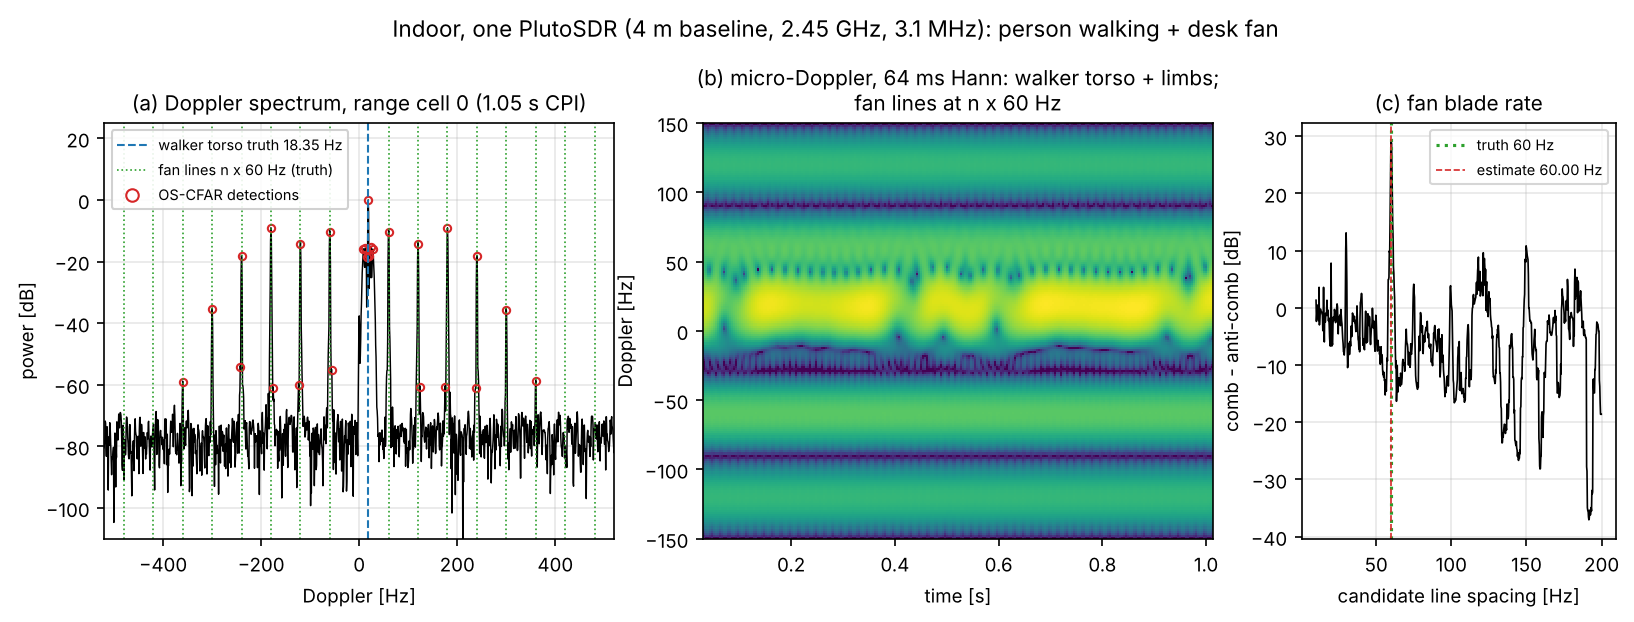
\includegraphics[width=\linewidth]{fig02_indoor.png}
\caption{Indoor. (a) Doppler spectrum of range cell 0 with OS-CFAR detections; the fan lines at $n\times60$\,Hz and the
walker's torso line and limb lines are resolved. (b) Spectrogram (64\,ms window). (c) Rotor line-spacing score.}
\end{figure}

\FloatBarrier
\needspace{12\baselineskip}
\subsection{Outdoor: quadcopter and person}
\begin{table}[htbp]
\centering\small
\caption{Outdoor results (one Pluto, \TcpiO\,ms CPI). Cells: \RresO\,m and \DresO\,Hz.}
\begin{tabular}{lccc}
\toprule
Quantity & Truth & Estimate & Error\\
\midrule
UAV excess range-sum & \UavRT\,m & \UavRE\,m & \UavRErr\,m (\UavRErrC\ cells)\\
UAV Doppler & \UavDT\,Hz & \UavDE\,Hz & \UavDErr\,Hz (\UavDErrC\ cells)\\
UAV range-sum rate & \UavVT\,m/s & \UavVE\,m/s & \\
UAV rotor line spacing & \UavBrMin--\UavBrMax\,Hz & \UavBrE\,Hz & inside the spread of the four rotors\\
Person Doppler (slow) & \PersDT\,Hz & \PersDE\,Hz & \PersDErr\,Hz (zero-Doppler notch bias)\\
Communication & & BER \BerO\ over \BitsO\ bits & EVM \EvmO\,dB\\
\bottomrule
\end{tabular}
\end{table}
\begin{figure}[htbp]
\centering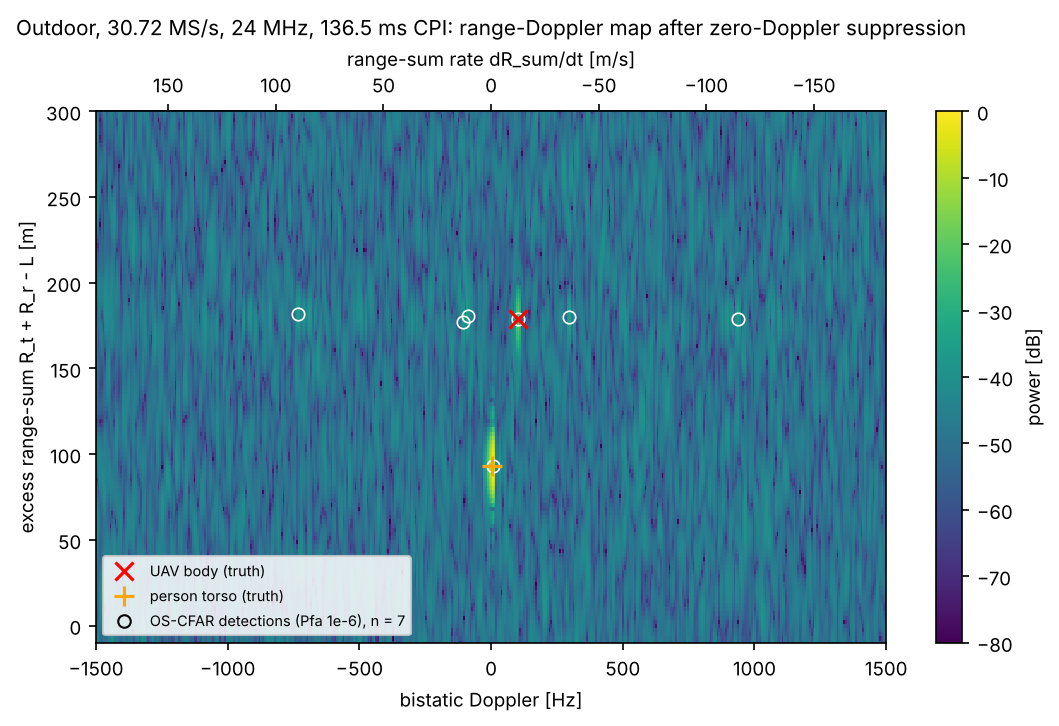
\includegraphics[width=0.82\linewidth]{fig03_outdoor_range_doppler.png}
\caption{Outdoor range-Doppler map after zero-Doppler suppression, with OS-CFAR detections ($P_{fa}=10^{-6}$). The
detections along the UAV's range cell are its rotor lines.}
\end{figure}
\begin{figure}[htbp]
\centering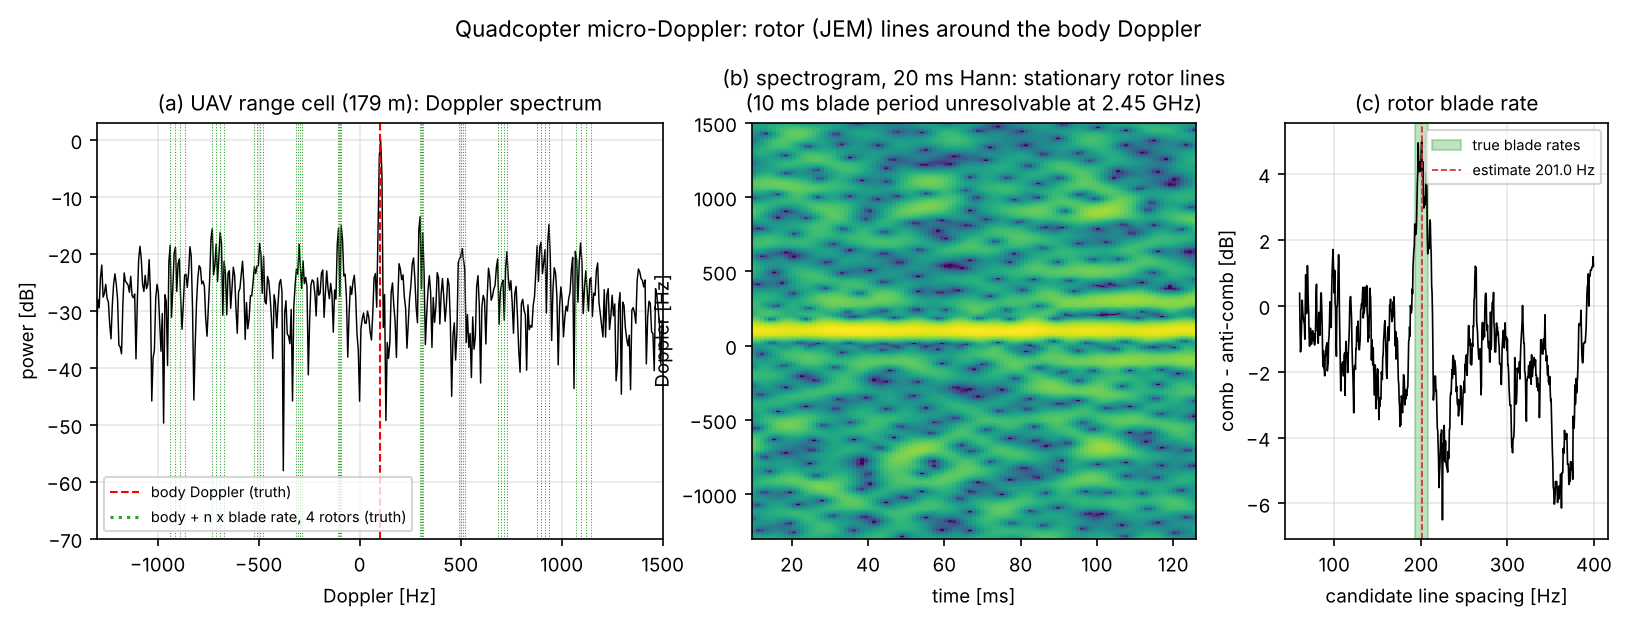
\includegraphics[width=\linewidth]{fig04_uav_micro_doppler.png}
\caption{UAV range cell: (a) Doppler spectrum with the rotor lines expected from the truth; (b) spectrogram;
(c) rotor line-spacing score. The four rotors' blade rates differ by 5\,Hz, below the \DresO\,Hz resolution.}
\end{figure}

\FloatBarrier
\needspace{12\baselineskip}
\subsection{Two separate PlutoSDRs}
\begin{table}[htbp]
\centering\small
\caption{Indoor walker with independent clocks (2\,ppm: CFO \TwoCfoT\,Hz, SFO 2\,ppm, $\beta=$\TwoLw\,Hz). Walker truth:
\TwoDT\,Hz, \TwoRT\,m.}
\footnotesize
\begin{tabular}{lccc}
\toprule
Processing & BER & Walker & Error\\
\midrule
One Pluto (shared clock), reference & \TwoOneBer & \TwoOneD\,Hz, SNR \TwoOneSnr\,dB & \TwoOneDErr\,Hz\\
Two Plutos, no correction & \TwoBerNone & \TwoWalkNone & --\\
Two Plutos, CFO correction only & \TwoCfoOnlyBer & excess range \TwoCfoOnlyR\,m & \TwoCfoOnlyRErr\,m (SFO uncorrected)\\
Two Plutos, CFO + direct-path referencing & \TwoRefBer & \TwoRefD\,Hz, \TwoRefR\,m, SNR \TwoRefSnr\,dB & \TwoRefDErr\,Hz, \TwoRefRErr\,m\\
\bottomrule
\end{tabular}
\end{table}
\noindent The CFO estimate is \TwoCfoE\,Hz (error \TwoCfoErr\,Hz).

\begin{table}[htbp]
\centering\small
\caption{Walker detection SNR [dB] versus relative LO phase-noise linewidth $\beta$ [Hz] and phase-reference smoothing.}
\begin{tabular}{l*{6}{c}}
\toprule
Smoothing $\backslash\ \beta$ & \SensHead\\
\midrule
\SensRows
\bottomrule
\end{tabular}
\end{table}
\begin{figure}[htbp]
\centering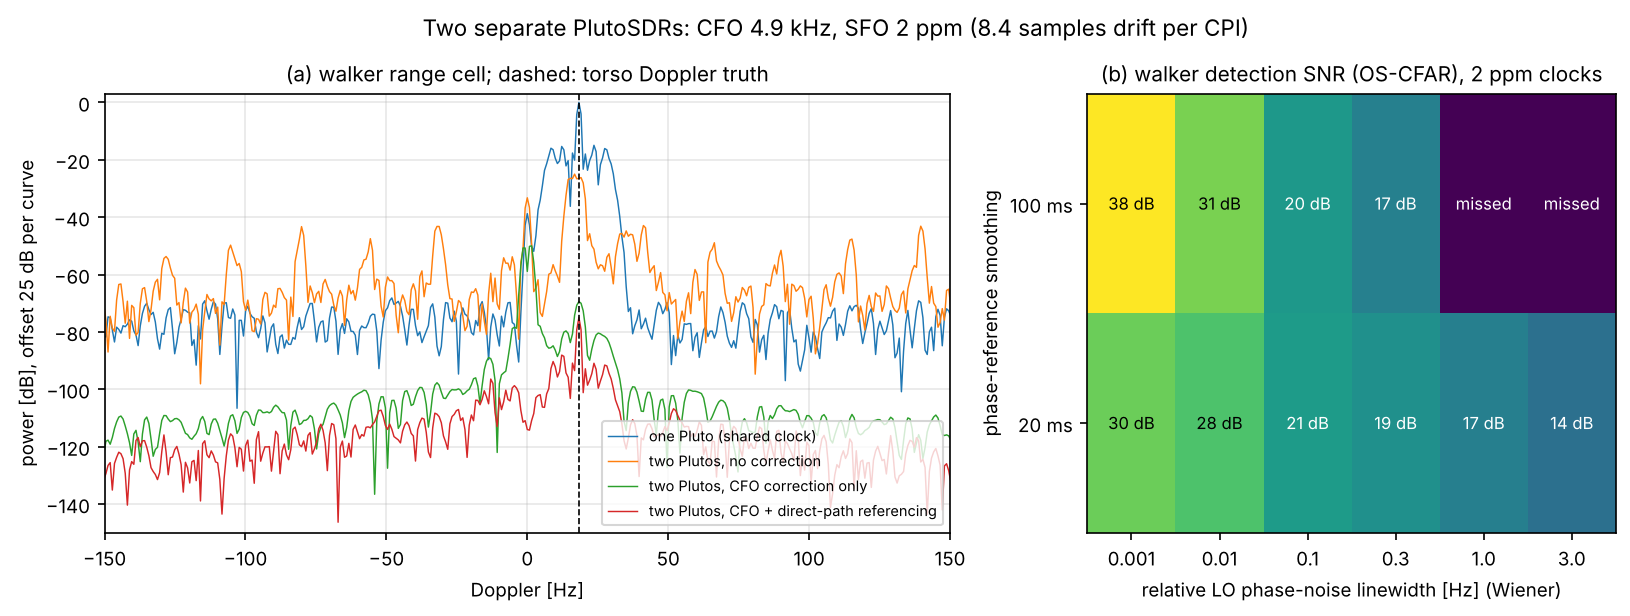
\includegraphics[width=\linewidth]{fig05_two_device_sync.png}
\caption{Two Plutos: (a) walker range cell under the four processing options; (b) sensitivity to phase noise.}
\end{figure}

\FloatBarrier
\needspace{12\baselineskip}
\subsection{Communication}
The same captures carry the data link. BER and EVM of both runs are listed in the indoor and outdoor result tables;
Fig.~\ref{fig:comm} shows the equalised symbols.
\begin{figure}[H]
\centering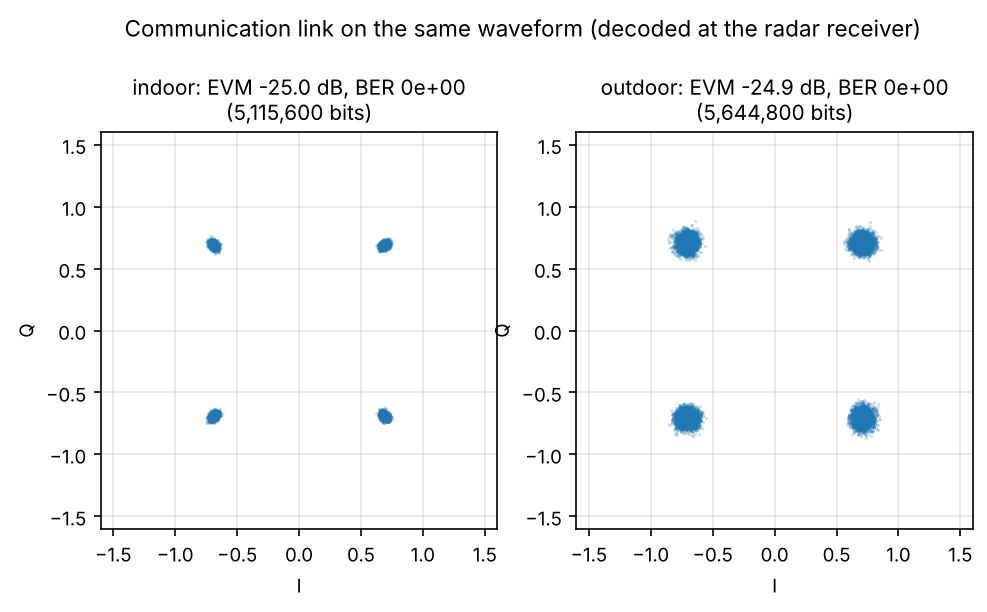
\includegraphics[width=0.62\linewidth]{fig06_comm_constellation.png}
\caption{Equalised QPSK symbols decoded at the radar receiver (first frame of each run).}\label{fig:comm}
\end{figure}

\FloatBarrier
\needspace{12\baselineskip}
\subsection{Monte Carlo: UAV detection versus distance}
\McTrials\ random tracks per distance (azimuth 30--150$^\circ$, height 20--60\,m, speed 3--12\,m/s, random heading),
outdoor configuration, OS-CFAR with $P_{fa}=10^{-6}$. A detection counts if it lies within $\pm2$ range cells and
$\pm3$ Doppler cells of the truth. The measured CFAR SNR is below the link-budget prediction mainly because of the Hann windows (about 1.8\,dB
per dimension) and of straddle loss. Where only a few tracks are detected, their SNR is biased upwards
(selection bias). The Doppler RMSE is larger at 50\,m than at 100--200\,m because close, fast tracks accelerate along
the line of sight: within one CPI their Doppler changes by a median of 1.9\,Hz and by up to 6.3\,Hz (0.86 cell) for
this track distribution, which widens and skews the peak.
\begin{table}[htbp]
\centering\small
\caption{Monte Carlo (\McTrials\ tracks per distance). RMSE over detected tracks only.}
\begin{tabular}{rccccc}
\toprule
Distance [m] & $P_D$ & Predicted SNR [dB] & Measured SNR [dB] & RMSE range [m] & RMSE Doppler [Hz]\\
\midrule
\McRows
\bottomrule
\end{tabular}
\end{table}
\begin{figure}[htbp]
\centering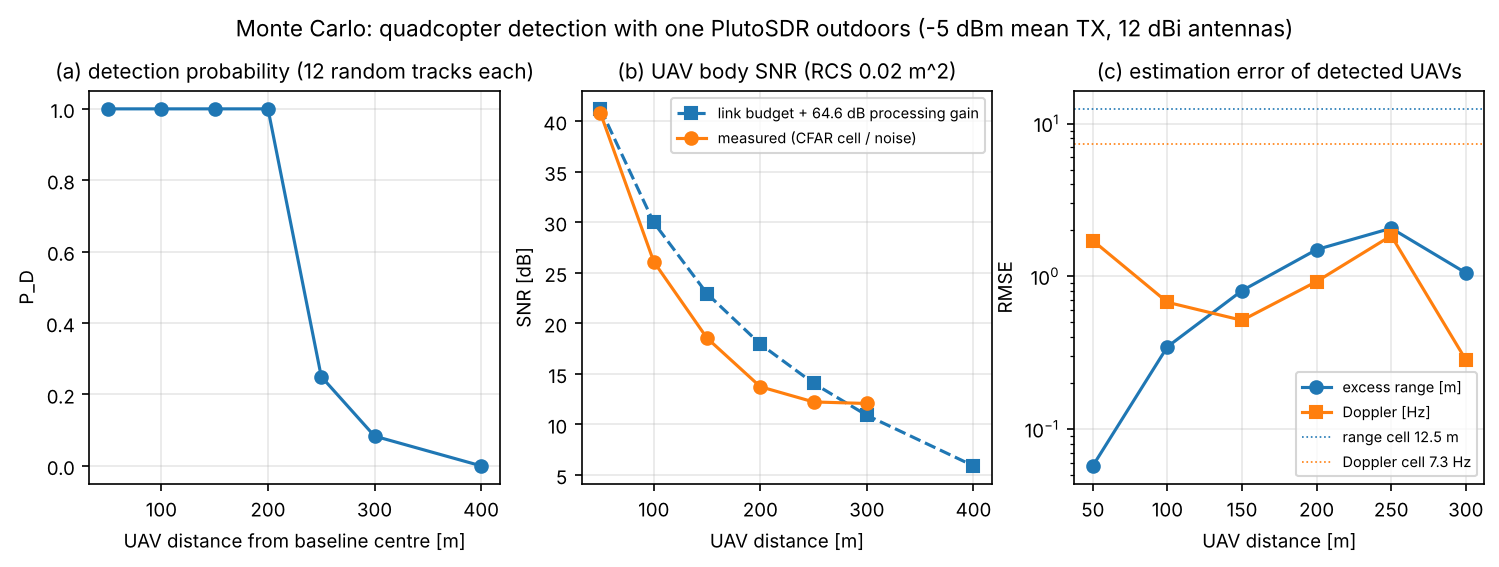
\includegraphics[width=\linewidth]{fig07_monte_carlo_uav.png}
\caption{Monte Carlo: detection probability, SNR and estimation error versus distance.}
\end{figure}

%======================================================================================
\section{Verification}
\subsection{Tests}
All tests pass (\code{python -m pytest}); the GNU Radio tests need GNU Radio~3.10 (with gr-iio and PyQt5) and are skipped
otherwise. The suite passes on Python~3.13 (numpy~2.5), on Ubuntu~24.04's Python~3.12 (numpy~1.26, scipy~1.11) and on
Python~3.10 with numpy~1.21, scipy~1.8 and matplotlib~3.5 (Ubuntu~22.04 versions); the simulation results agree on all
three to within $2\times10^{-7}$ (relative; float32 rounding). The hardware code paths are tested against simulated drivers (\code{tests/fakes}): a stand-in for
\code{pyadi-iio}'s \code{adi.Pluto} and for gr-iio's PlutoSDR Source and Sink. Both enforce the real drivers' limits
(gain and attenuation ranges, int16 TX range, cyclic-buffer rules, one-buffer pushes) and record every configuration call;
the simulated RX samples come from the channel simulator, driven by the samples the code under test transmitted.
\begin{small}
\begin{longtable}{p{0.40\linewidth}p{0.54\linewidth}}
\toprule
Test & What it checks\\
\midrule
\endhead
%%TESTS_TABLE%%
\bottomrule
\end{longtable}
\end{small}

\subsection{Defects found and fixed during development}
\begin{enumerate}
\item ADC clipping (gain set on the direct path only) produced false Doppler lines at the TX-buffer rate.
\item The empty DC subcarrier produced a $-52$\,dB range pedestal.
\item Cell-averaging CFAR missed the walking person (extended-target masking); replaced by OS-CFAR.
\item The rotor-rate estimator locked onto $3\times$ the fan rate; fixed with the multi-fraction anti-comb.
\item Frame synchronisation could lock onto the next TX buffer, wasting up to one buffer of the CPI.
\item The embedded GNU Radio block requested more input than a stream buffer holds and stalled the scheduler.
\item Review findings: the TX power assumption was about 10\,dB too optimistic and has been corrected (all results
in this report use the corrected value); the TX digital level differed by 6\,dB between the pyadi and GNU Radio paths;
the RX gain range in the GUI was wrong; the phase-noise conversion missed a factor of 2; a flowgraph variable depended
on the working directory at compile time; two BER entries of a report table were typed rather than generated.
\item Second review: the Ubuntu set-up installed libiio bindings incompatible with Ubuntu's libiio (fixed by using
\code{python3-libiio}); package minimums forced pip to replace Ubuntu's numpy and matplotlib (lowered and tested on
the Ubuntu~22.04 and 24.04 versions); the RX-record flowgraph wrote into a folder missing from a fresh clone; the capture
script did not validate gain and attenuation before configuring the radio.
\end{enumerate}

%======================================================================================
\section{Hardware validation plan}\label{sec:plan}
\begin{tabularx}{\linewidth}{lL}
\toprule
E0 & Cable loop-back through 50\,dB attenuation: sync, BER, EVM, system delay, TX power (power meter).\\
E1 & Static scene: no detections, dynamic range, absence of buffer-rate lines.\\
E2 & Pendulum (metal plate): period and peak Doppler against \code{scripts/predict.py}.\\
E3 & Walking person on a taped line with a stopwatch: torso Doppler against the prediction from geometry.\\
E4 & Desk fan with a reference rpm: rotor line spacing; point-scatterer lines versus real blade flashes.\\
E5 & Two Plutos (optionally SDR++ as the receiver): CFO estimate, BER, walker error.\\
E6 & Outdoor UAV with GPS ground truth (only with a pilot and permission).\\
\bottomrule
\end{tabularx}

%======================================================================================
\section{Limitations}
\begin{itemize}
\item Indoors the range-sum resolution is \RresI\,m: targets are separated by Doppler only.
\item Targets slower than about one Doppler cell are attenuated and biased by the zero-Doppler notch.
\item The simulation uses point scatterers and isotropic antenna gains. Multipath, body shadowing, blade flashes,
blade-tip ICI, PA non-linearity, IQ imbalance, LO leakage and USB sample drops are not modelled (the last is
detected in recordings).
\item The TX power, noise figure, isolation and RCS values are assumptions (Table~\ref{tab:assumptions}).
\item The capture scripts and the GNU Radio hardware flowgraphs are tested against simulated drivers, not yet on a real
PlutoSDR; the SDR++ GUI procedure is untested.
\end{itemize}

\begin{thebibliography}{9}\small
\bibitem{sturm2011} C.~Sturm, W.~Wiesbeck, ``Waveform design and signal processing aspects for fusion of wireless
communications and radar sensing,'' \emph{Proc.\ IEEE}, vol.~99, no.~7, 2011.
\bibitem{vandebeek1997} J.-J.~van de Beek, M.~Sandell, P.\,O.~B\"orjesson, ``ML estimation of time and frequency offset
in OFDM systems,'' \emph{IEEE Trans.\ Signal Process.}, vol.~45, no.~7, 1997.
\bibitem{rohling1983} H.~Rohling, ``Radar CFAR thresholding in clutter and multiple target situations,''
\emph{IEEE Trans.\ Aerosp.\ Electron.\ Syst.}, vol.~19, no.~4, 1983.
\bibitem{chen2011} V.\,C.~Chen, \emph{The Micro-Doppler Effect in Radar}, Artech House, 2011.
\bibitem{ad9363} Analog Devices, \emph{AD9363 RF Agile Transceiver data sheet}, Rev.~D.
\bibitem{adiTx} Analog Devices, ``ADALM-PLUTO: transmit,'' \url{https://wiki.analog.com/university/tools/pluto/users/transmit}.
\bibitem{griio} GNU Radio 3.10.9.2, gr-iio \code{fmcomms2\_sink\_impl.cc} and \code{fmcomms2\_source\_impl.cc}.
\bibitem{mathworksPluto} MathWorks, ``PlutoSDR radio parameters and supported ranges,''
\url{https://www.mathworks.com/help/comm/plutoradio/ug/plutoradio-parameters-and-supported-ranges.html}.
\end{thebibliography}
\end{document}
